В данной работе в качестве базового алгоритма всех алгоритмов классификации (см. разделы~\ref{random_forest},
\ref{ada}, \ref{extra}) в данной работе были выбраны деревья решений 
(Decision Trees), тестирование и оценка модели производилась на основе 10-фолдовой кросс-валидации.

Деревья решений (Decision Trees) или деревья принятия решений --- является одним из наиболее популярных
методов решения задач классификации, регрессии и прогнозирования. Впервые деревья решений были предложены Ховилендом и Хантом (Hoveland, Hunt) 
в конце 50-х годов прошлого века и в наиболее простом виде представляют собой совокупность правил в иерархической 
структуре. Основа такой структуры --- это ветвление при проверке условий (<<Да>> --- <<Нет>>).~\cite{data_mining} 

Кросс-валидация (cross-validation) или перекрестная проверка --- 
процедура скользящего контроля, предотвращающая ошибку 3-го рода, совершаемую 
при принятии методики испытаний на основе ошибочного допущения. Используется в качестве метода оценки
аналитической модели и ее поведения на независимых данных. При оценке модели имеющиеся в наличии 
данные разбиваются на k частей. Затем на k−1 частях данных производится обучение модели, 
а оставшаяся часть данных используется для тестирования. Процедура повторяется k раз; 
в итоге каждая из k частей данных используется для тестирования. 
В результате получается оценка эффективности выбранной модели с наиболее равномерным 
использованием имеющихся данных.~\cite{crossval}




\subsection{Random Forest}\label{random_forest}
Алгоритм классификации Random Forest Classifier строится на двух базовых принципах: 
\begin{itemize}
  \item bagging --- мета-алгоритм в машинном обучении, при котором на основе большого числа <<слабых>> классификаторов (в данном случае деревьев решений) строится один <<сильный>> классификатор (рис.~\ref{forest:forest});
  \item метод случайных подпространств.
\end{itemize}

Преимущества данного алгоритма классификации:
\begin{itemize}
  \item способность эффективно обрабатывать данные с большим числом признаков и классов;
  \item нечувствительность к масштабированию (к любым монотонным преобразованиям) значений признаков;
  \item существует методы оценивания значимости отдельных признаков в модели;
  \item внутренняя оценка способности модели к обобщению (тест out-of-bag);
  \item высокая параллелизуемость и масштабируемость.
\end{itemize}

Недостатки алгоритма Random Forest Classifier:
\begin{itemize}
  \item алгоритм склонен к переобучению на некоторых задачах, особенно на зашумленных, однако для избежания переобучения используется энтропия Шеннона или коэффициент прироста информации (англ. Gain);
  \item большой размер получаемых моделей приводит к существенным затратам памяти на хранение деревьев, однако данный недостаток решается повышением вычислительных мощностей и распараллеливанием вычислений.~\cite{random_forest}
\end{itemize}

\begin{figure}[h!]
\center{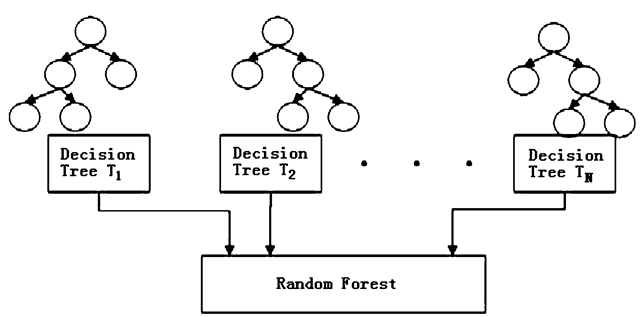
\includegraphics[width=0.7\linewidth]{forest}}
\caption{ Random Forest Classifier }
\label{forest:forest}
\end{figure} 

 

\subsection{AdaBoost}\label{ada}
Алгоритм AdaBoost (сокр. от adaptive boosting)~\cite{ada_boost} является мета-алгоритмом, в процессе обучения 
строит композицию из базовых алгоритмов обучения для улучшения их эффективности.

Достоинства:
\begin{itemize}
 \item хорошая обобщающая способность --- в реальных задачах (не всегда, но часто) удаётся строить композиции, 
превосходящие по качеству базовые алгоритмы, при этом обобщающая способность может улучшаться (в некоторых задачах) 
по мере увеличения числа базовых алгоритмов;
 \item простота реализации;
 \item время построения композиции практически полностью определяется временем обучения базовых алгоритмов.
\end{itemize}


Недостатки алгоритма классификаций AdaBoost:
\begin{itemize}
 \item склонен к переобучению при наличии значительного уровня шума в данных;
 \item требует достаточно длинных обучающих выборок;
 \item бустинг может приводить к построению громоздких композиций, состоящих из сотен алгоритмов, 
 такие композиции исключают возможность содержательной интерпретации, требуют больших объёмов памяти 
 для хранения базовых алгоритмов и существенных затрат времени на вычисление классификаций.
\end{itemize}

\subsection{ExtraTrees}\label{extra}
Алгоритм ExtraTrees (Extremly Randomized Trees) является модификацией 
алгоритма Random Forest Classifier (см. раздел~\ref{random_forest}), но отличается еще более рандомизированным
разделением входного набора данных на подвыборки. Как правило, результаты работы данного алгоритма
схожи с результатами Random Forest Classifier, однако в определенных случаях могут давать улучшение
точности классификации.~\cite{extra_trees}

